\clearpage
\section{角色胶囊的三种取值}

给一个新实体加上 3D 胶囊碰撞体，总长是 1.80 米。打开潮汐维修站，选中玩家，同一个字段是 1.84 米。前一个数由 C++ 组件的初始值决定，后一个数保存在场景里。假设想试试把玩家调到 1.90 米，还会出现第三个数。只有保存修改后，下一次打开场景才会读到它。

\begin{center}
\small\renewcommand{\arraystretch}{1.32}
\begin{tabularx}{.96\linewidth}{@{}L{25mm}L{19mm}Y@{}}
\toprule
& \textbf{总长} & \textbf{读数的位置}\\
\midrule
引擎默认值 & 1.80 米 & 新建胶囊组件，读取其中的 \code{Height}。MCP 查原生程序导出的默认值表。\\
场景当前值 & 1.84 米 & 读取维修站场景中编号 1101 的实体，再取它的胶囊总长。这是此版本的保存值。\\
本次候选值 & 1.90 米 & 由这次预览传入。可以先比较差别，再决定是否保存。\\
\bottomrule
\end{tabularx}
\end{center}

\begin{figure}[H]\centering
\begin{minipage}[c]{.25\linewidth}\centering
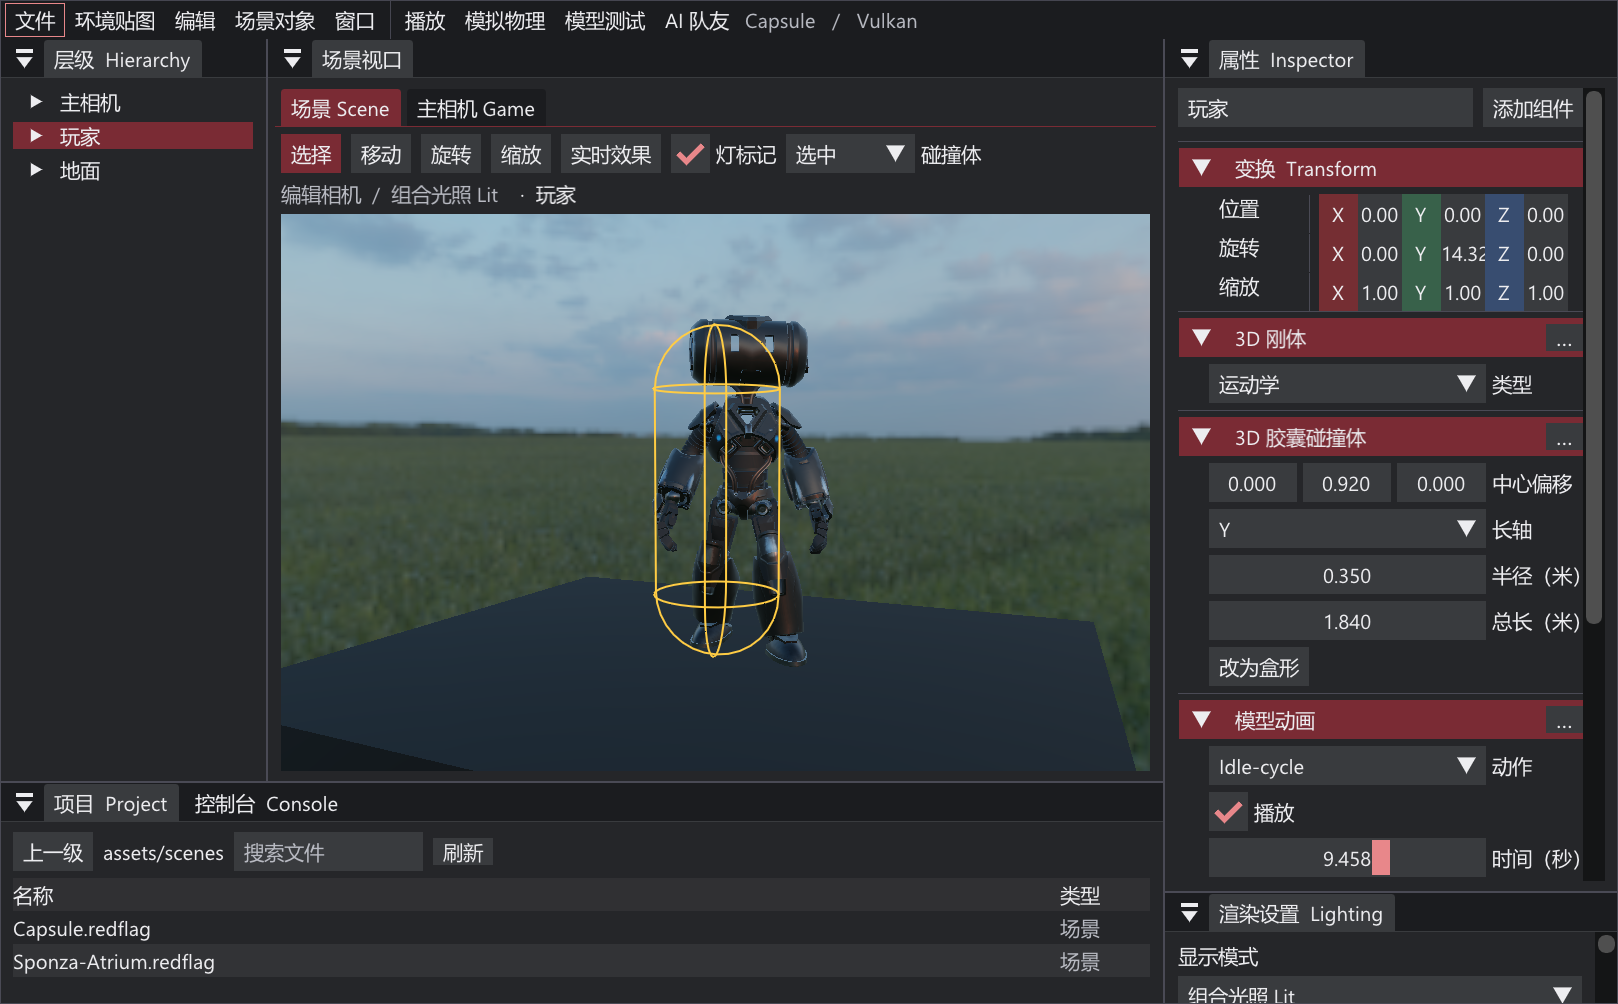
\includegraphics[viewport=582 280 915 742,clip,height=35mm]{../../../output/validation/packaged-watt/ground-contact/editor/before.png}
\end{minipage}\hspace{3mm}%
\begin{minipage}[c]{.63\linewidth}
\caption{Forge 中选中角色的实拍局部。黄色线圈勾出场景为角色配置的碰撞体，总长从上端圆顶量到下端圆底。旁边伸出的手臂仍然属于角色模型。}
\end{minipage}
\end{figure}

在 Forge 里，用户点的是“总长”，源码里这个成员叫 \code{Height}。引擎把它的名称、单位和读写方法放在一起，供工具按名字查找。程序可以在运行时问“这个组件有哪些字段、怎样读取其中一个”，这就是这里用到的\textbf{反射}。字段的读方法需要传入实体，同一个方法既能读玩家，也能读瓦特。

\codewhere{C++ 调用示例}{Redflag/src/Redflag/Scene/ComponentReflection.h}{FindComponent、FindField 与 Field::Read}
\begin{lstlisting}
const auto* capsule = Reflection::FindComponent("CapsuleCollider3DComponent");
const auto* height = capsule->FindField("Height");
auto current = height->Read(player);  // (*@玩家缺少这个组件时，结果为空。@*)
\end{lstlisting}

原作者定尺寸时用过不同依据。站立总长 1.84 米沿用旧碰撞盒的两倍半高。蹲行则以每秒 120 个姿势测量，模型头顶最高到 1.33088 米，取到厘米后得到 1.33 米。倒地时背甲最低处到身体最高处约 0.658 米，横放胶囊取一半作为半径，约 0.33 米。测量按模型原尺寸进行，瓦特的 0.96 倍场景缩放另算。取值记录保存在场景旁，作者改过尺寸以后，仍能查到最初的依据。

\readings{\src{Redflag/src/Redflag/Scene/Components.h}{C++ 组件初始值}\quad
\src{RedflagForge/assets/scenes/Watt-Station.redflag}{维修站场景}\quad
\src{RedflagForge/assets/scenes/Watt-Station.tuning.yaml}{取值记录}\quad
\src{output/validation/packaged-watt/ground-contact/model.json}{动作测量}}

\clearpage
\section{组件字段的修改与撤销}

把胶囊总长从 1.84 米试调到 1.90 米时，Forge 可以直接询问正在编辑的实体。MCP 面对的是磁盘上的场景，先按实体编号和字段名读值，再根据引擎的字段说明检查候选值。两处共用的说明保存在 \src{Redflag/src/Redflag/Scene/ComponentFields.json}{ComponentFields.json}。它包含字段类型和长度单位，也记着胶囊总长至少等于直径。角色在游戏中倒地、暂停时横放的那个胶囊，属于本局的场景副本。

\codewhere{MCP 调用示例}{scripts/redflag_mcp/server.py}{inspect\_scene\_fields 与资产修改工具}
\begin{lstlisting}
review = inspect_scene_fields("Watt-Station.redflag", "1101",
    "CapsuleCollider3DComponent", proposed={"Height": 1.90})
ops = review["operations"]         # (*@保存了实体编号、字段名、原值和候选值。@*)
change = propose_asset_change("(*@试调站立碰撞体高度@*)", ops)
apply_asset_change(change["id"])   # (*@重新读场景，核对原值后写入。@*)
\end{lstlisting}

如果另一位作者先把同一项改成 1.86 米，原提案会停下来，并显示查到的新值。若对方只改了角色名字，保存这项高度时会保留新名字。撤销时传入同一编号和 \code{undo=True}，工具再次比较该字段。游戏要从保存的场景重新开局，才能用新身高测试通道是否足够宽。

Piccolo 的 \code{RigidBodyShape} 很适合对照阅读。打开其刚体资源头文件，形状的局部变换和几何体引用标了 \code{META(Enable)}。模板为选中的成员生成取得名称、读成员、写成员的函数，再登记到类型上。调用方拿到 \code{FieldAccessor} 后，就能操作某个具体实例。Redflag 当前为盒形、胶囊碰撞体和 3D 刚体登记字段，生成普通 C++ 成员绑定。一次写入先在组件副本上检查尺寸，检查通过再改原成员。物理形状仍由原来的组件和物理系统负责。

在仓库根目录，用 MCP 的 Python 环境运行 \src{tests/check_component_authoring.py}{check\_component\_authoring.py}，会在临时维修站里实际完成预览、保存和撤销，同时调整半径和总长，复查作者改名、旧场景缺字段以及同字段冲突。运行 \code{tests/run\_scene\_tests.cmd --component-reflection} 可以验证原生实体的读写与默认值。贴墙测试另测的是角色在两个半径下停在哪里。移动检测取角色半径的 0.9 倍是既有经验系数，这次测试没有比较多个系数。

\readings{\href{https://github.com/BoomingTech/Piccolo/blob/f5053707fed4d3f94d270a436fb0d3a8ae54e3e5/engine/source/runtime/resource/res_type/components/rigid_body.h}{Piccolo · 刚体资源}\quad
\href{https://github.com/BoomingTech/Piccolo/blob/f5053707fed4d3f94d270a436fb0d3a8ae54e3e5/engine/template/commonReflectionFile.mustache}{生成模板}\quad
\href{https://github.com/BoomingTech/Piccolo/blob/f5053707fed4d3f94d270a436fb0d3a8ae54e3e5/engine/source/runtime/core/meta/reflection/reflection.h}{字段访问器}\quad
\src{Redflag/src/Redflag/Scene/ComponentReflection.cpp}{Redflag 成员绑定}\quad
\src{output/validation/packaged-watt/ground-contact/radius.json}{贴墙实测}}
